\documentclass[11pt,a4paper,dvipdfmx]{article}
%\documentclass[autodetect-engine,dvipdfmx-if-dvi,ja=standard]{bxjsarticle}

\usepackage[utf8]{inputenc}
\usepackage{lmodern}
\usepackage[T1]{fontenc}
\usepackage[noBBpl]{mathpazo}
%\linespread{1.05}
\usepackage{mathtools, amsmath, amssymb, amsthm}
\usepackage{amsfonts}
\usepackage{braket}
%\usepackage{amssymb}
\usepackage{url}

%% citation
\usepackage[longnamesfirst]{natbib}

%
\theoremstyle{plain}
\newtheorem{thm}{Thm.}[section]
\newtheorem{lem}{Lem.}[section]
\newtheorem{cor}{Cor.}[section]
\newtheorem{prop}{Prop.}[section]
\newtheorem{df}{Def.}[section]
\newtheorem{eg}{e.g.}[section]
\newtheorem{rem}{Rem.}[section]
%

\usepackage{listings,jlisting}
\lstset{%
language={python},%
basicstyle={\ttfamily\footnotesize},%ソースコードの文字を小さくする
frame={single},
commentstyle={\footnotesize\itshape},%コメントアウトの文字を小さくする
breaklines=true,%行が長くなったときの改行。trueの場合は改行する。
numbers=left,%行番号を左に書く。消す場合はnone。
xrightmargin=3zw,%左の空白の大きさ
xleftmargin=3zw,%右の空白の大きさ
stepnumber=1,%行番号を1から始める場合こうする(たぶん)
numbersep=1zw,%行番号と本文の間隔。
}

%\usepackage[dvipdfmx]{graphicx}
%% color packageとdvipdfmxは相性が悪いらしい
%% https://qiita.com/zr_tex8r/items/442b75b452b11bee8049
\usepackage{graphicx}


\usepackage[left=2cm,right=2cm,top=2cm,bottom=2cm]{geometry} %This changes the margins.
\usepackage{float}
%\author{Kyohei Okumura}
\global\long\def\T#1{#1^{\top}}

\newcommand{\id}{\textnormal{id}}
\newcommand{\R}{\mathbb{R}}
\newcommand{\N}{\mathbb{N}}
\newcommand{\Q}{\mathbb{Q}}
\newcommand{\Z}{\mathbb{Z}}
\newcommand{\C}{\mathbb{C}}
\newcommand{\mF}{\mathcal{F}}
\newcommand{\mG}{\mathcal{G}}
\newcommand{\mA}{\mathcal{A}}
\newcommand{\mB}{\mathcal{B}}
\newcommand{\mC}{\mathcal{C}}
\newcommand{\mD}{\mathcal{D}}
\newcommand{\mL}{\mathcal{L}}
\newcommand{\mM}{\mathcal{M}}
\newcommand{\mO}{\mathcal{O}}
\newcommand{\mP}{\mathcal{P}}
\newcommand{\mS}{\mathcal{S}}
\newcommand{\mT}{\mathcal{T}}
\newcommand{\mV}{\mathcal{V}}
\renewcommand{\Re}{\mathrm{Re}}
\renewcommand{\hat}{\widehat}
\renewcommand{\tilde}{\widetilde}
\renewcommand{\bar}{\overline}
\renewcommand{\epsilon}{\varepsilon}
% \renewcommand{\span}{\mathrm{span}}
\newcommand{\defi}{\stackrel{\Delta}{\Longleftrightarrow}}
\newcommand{\equi}{\Longleftrightarrow}
\newcommand{\s}{\succsim}
\newcommand{\p}{\precsim}
\newcommand{\join}{\vee}
\newcommand{\meet}{\wedge}
\newcommand{\1}{\mbox{1}\hspace{-0.25em}\mbox{l}}

\DeclareMathOperator{\Var}{Var}
\DeclareMathOperator{\Cov}{Cov}
\DeclareMathOperator{\sgn}{sgn}
\DeclareMathOperator{\Card}{Card}
\DeclareMathOperator{\supp}{supp}
\DeclareMathOperator{\Log}{Log}
\DeclareMathOperator{\spn}{span}

\newcommand{\indep}{\mathop{\perp\!\!\!\!\perp}}

\usepackage{color}
\newcommand{\kcomment}[1]{{\textcolor{blue}{#1}}}
\newcommand{\ocomment}[1]{{\textcolor{red}{#1}}}


\begin{document}
\title{SML HW1}
\author{29-176004 奥村 恭平{\footnote{E-mail: kyohei.okumura@gmail.com}
\footnote{東京大学大学院 経済学研究科 M2}
}}
\date{\today}
\maketitle

%%%%%%%%%%%%%%%%%%%%%%%%%%%%%%%%%%%%%%%%%%%%%%%%%%%%%%%%%%%

\section{パターン認識の実例: 対テロ警備}
今,東京と鳥取という2つの街をテロリストが攻めようとしており,警察はテロリストから街を守ろうとしている状況を考える.$x$で,テロリストに対する情報パターン(過去の活動・国際情勢 etc.)を表すとする.
警察の人員には限りがあるので,どちらか一つの街しか守れないとする.
$p(y \mid x )$で,「パターン$x$の下で,テロリストが街$y$を攻める確率」とする.$x$を所与とし,いま,
$$p(y \mid x) :=
\begin{cases}
	0.7 & (y = \text{鳥取}) \\
	0.3 & (y = \text{東京})
\end{cases}
$$
だったとする.

損失を以下のように定義する.
$$
l_{\text{東京}, \text{鳥取}} := -10000000, \ 
l_{\text{鳥取}, \text{東京}} := -500000
$$
これは,東京の方が鳥取より人口が多いことに対応している.これは確かに,誤って識別した場合の損失がカテゴリによって異なるようなパターン認識の実例になっている.

このとき,例えば,期待損失を計算してみると,
\begin{align*}
	R(y = \text{東京} \mid x) &= 0.3 \cdot (- 10000000) = - 3000000 \\
	R(y = \text{鳥取} \mid x) &= 0.7 \cdot (- 500000) = - 350000
\end{align*}
となり,$\hat{y} := \arg \min_y R(y \mid x) = \text{東京}$となることがわかる.


\section{計算機演習}
\subsection{宿題1}
\begin{lstlisting}[caption=correlation]
import numpy as np
n = 1000

x = np.random.randn(n)
y1 = x + np.random.randn(n)
y2 = -x + np.random.randn(n)
y3 = np.random.randn(n)
y4 = x**2 + np.random.randn(n)

print(np.corrcoef(x, y1)[0, 1])
print(np.corrcoef(x, y2)[0, 1])
print(np.corrcoef(x, y3)[0, 1])
print(np.corrcoef(x, y4)[0, 1])

Output:
0.729195186123
-0.731054853932
0.020960020396
0.0511090973279
\end{lstlisting}

相関係数の正負は大まかには,プロットしたときに散布図が右上がりか右下がりかを表している.しかし,3つ目と4つ目の例を比べてみるとわかるように,相関係数が低いことは,二つの変量の間に規則的な関係がないことを必ずしも意味しない.(4つ目の例においては,$x,y$の間の相関係数はほぼ0だが,$y$は「$x$の2乗 + 誤差項」という形で生成されており,明らかに両者の間には規則的な関係がある.しかし,相関係数はこの関係性までは捉えられない.)

\subsection{宿題2}
以下のようなコードを用いて,二次元正規分布の密度関数の等高線をプロットした.言語はpython.

\begin{lstlisting}[caption=2d Gaussian]
import numpy as np
import matplotlib.pyplot as plt
from mpl_toolkits.mplot3d import axes3d
from matplotlib import cm

fig = plt.figure()
ax = fig.add_subplot(111, projection='3d')

x = y = np.arange(-5, 5, 0.1)
X, Y = np.meshgrid(x, y)

mu = np.array([0,0])

sigma = np.array([[2, 1], 
                  [1, 4]])

det = np.linalg.det(sigma)
inv_sigma = np.linalg.inv(sigma)

def gauss_2d(x, y):
    x_c = np.array([x, y]) - mu
    return np.exp(- x_c.dot(inv_sigma).dot(x_c[np.newaxis, :].T) / 2.0) / (2*np.pi*np.sqrt(det))

Z = np.vectorize(gauss_2d)(X, Y)

ax.plot_surface(X, Y, Z, rstride=1, cstride=1, cmap=cm.coolwarm)
plt.show()
\end{lstlisting}

\begin{figure}[H]
  \centering
  \begin{minipage}{0.48\hsize}
    \centering
    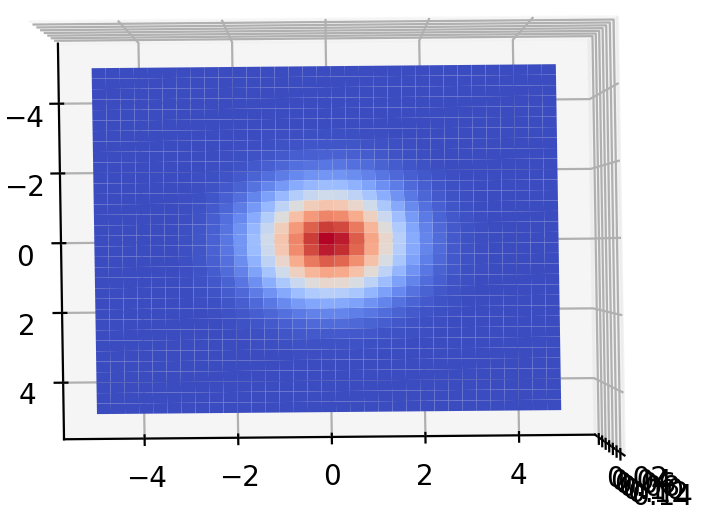
\includegraphics[height=6cm]{image/Figure_1.png}
    \caption{$\Sigma_1$}
    \label{fig:s2_prf_1}
  \end{minipage}
  \begin{minipage}{0.48\hsize}
    \centering
    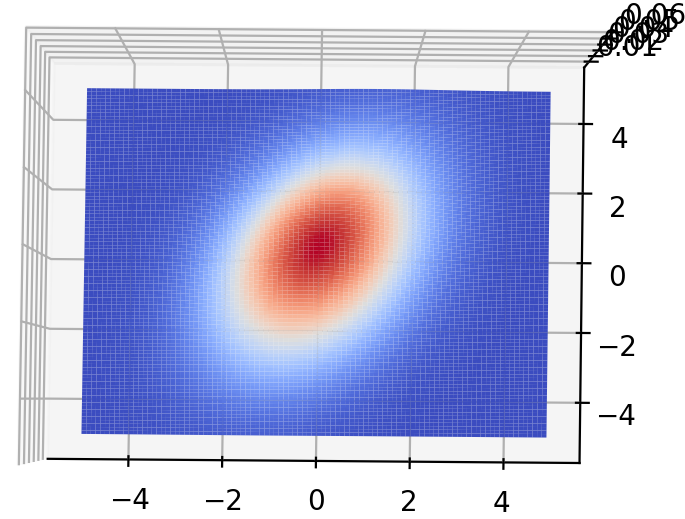
\includegraphics[height=6cm]{image/Figure_2.png}
    \caption{$\Sigma_2$}
    \label{fig:s2_prf_2}
  \end{minipage}
\end{figure}

上の図は,それぞれ,以下のように分散共分散行列を定めた場合の等高線の図である.
$$
\Sigma_1 := \left[
\begin{matrix}
	1 & 0 \\
	0 & 1
\end{matrix}
\right],
\quad
\Sigma_2 := \left[
\begin{matrix}
	2 & 1 \\
	1 & 4
\end{matrix}
\right].
$$

$\Sigma_2$に対応するグラフに着目する.
計算すると,$\Sigma_2^{-1}$の固有値は$\lambda_1 := 0.63060194,  \lambda_2 :=0.22654092$,対応する固有ベクトルは,
$x_1 := [0.92387953,-0.38268343]^\top, x_2 := [0.38268343, 0.92387953]^\top$となる.
\begin{itemize}
	\item 確率密度関数の裾野が,固有ベクトルの方向に向かって伸びている(等高線の楕円の軸が固有ベクトルを座標軸とみたものになっている)こと.
	\item 固有値が大きい固有ベクトルに対応する方向ほど,山の傾斜が急であること.
\end{itemize}
が観察される.以下,任意の分散共分散行列に対して,これらの性質(*)が成立することをもう少しキチンと示す.

簡単のため,$\mu = 0$とする.$\Sigma$を$2 \times 2$の半正定値対称行列とし,固有値を$\lambda_1 \geq \lambda_2 \geq 0$, 対応する固有ベクトル(長さ1に正規化済み)を$\phi_1, \phi_2$とする.いま,$x \in \R^2$を任意に固定する.固有ベクトルは基底を為すので,
$$
x = x_1 \phi_1 + x_2 \phi_2
$$
と表せることに注意すると,$\Sigma = \lambda_1 \phi_1 \phi_1^\top + \lambda_2 \phi_2 \phi_2^\top$であることを用いると,
$$
x^\top \Sigma x = x_1^2 \lambda_1 + x_2^2 \lambda_2
$$
となることが簡単な計算により示せる.

二次元正規分布の密度関数の,指数関数の中身の部分に着目する:
$$
-\frac{1}{2}x^\top \Sigma^{-1} x = - \frac{1}{2}(x_1^2 \lambda_1 + x_2^2 \lambda_2)
$$
これは,(*)が確かに成立することを示している.例えば,$x$の$\phi_1$成分$x_1$が大きくなると,$\lambda_1$に対応する速さで確率密度関数の値は減少する.



\end{document}